\documentclass[12pt,a4paper]{article}

% ============================
% Pacotes
% ============================
\usepackage[a4paper,margin=2.5cm]{geometry}
\usepackage[brazil]{babel}
\usepackage[utf8]{inputenc}
\usepackage[T1]{fontenc}
\usepackage{graphicx}
\usepackage{amsmath,amssymb}
\usepackage{siunitx}
\usepackage{hyperref}
\usepackage{float}
\usepackage{algorithm}
\usepackage{algpseudocode}
\usepackage{fancyhdr}
\usepackage{caption}
\usepackage{subcaption}
\usepackage{titlesec}
\usepackage{enumitem}
\usepackage{xcolor}
\usepackage{booktabs}
\usepackage{setspace}
\usepackage{newtxtext,newtxmath} % Fonte Times profissional

% ============================
% Cabeçalho e rodapé
% ============================
\setlength{\headheight}{15pt}
\pagestyle{fancy}
\fancyhf{}
\fancyhead[L]{Universidade Federal de Minas Gerais}
\fancyhead[R]{Programa de Pós-Graduação em Engenharia Elétrica}
\fancyfoot[C]{\thepage}

% ============================
% Títulos e espaçamento
% ============================
\titleformat{\section}{\bfseries\Large}{\thesection.}{0.5em}{}
\titleformat{\subsection}{\bfseries\large}{\thesubsection.}{0.5em}{}
\setlength{\parskip}{0.6em}
\onehalfspacing

% ============================
% Dados do relatório
% ============================
\newcommand{\universidade}{Universidade Federal de Minas Gerais}
\newcommand{\departamento}{Escola de Engenharia}
\newcommand{\curso}{Programa de Pós-Graduação em Engenharia Elétrica}
\newcommand{\disciplina}{Planejamento de Movimento de Robôs}
\newcommand{\titulo}{Trabalho Final}
\newcommand{\autor}{Pedro Antonio de Souza Campos Rodrigues}
\newcommand{\professor}{Prof. Luciano C. A. Pimenta}
\newcommand{\local}{Belo Horizonte -- MG}
\newcommand{\dataentrega}{3 de julho de 2026}

% ============================
% Capa 
% ============================
\begin{document}
\begin{titlepage}
    \begin{center}
    
    % ====== Logos ======
    \vspace*{-1cm}
    
\includegraphics[width=3.2cm]{figures/Logo_UFMG.png}\hfill
    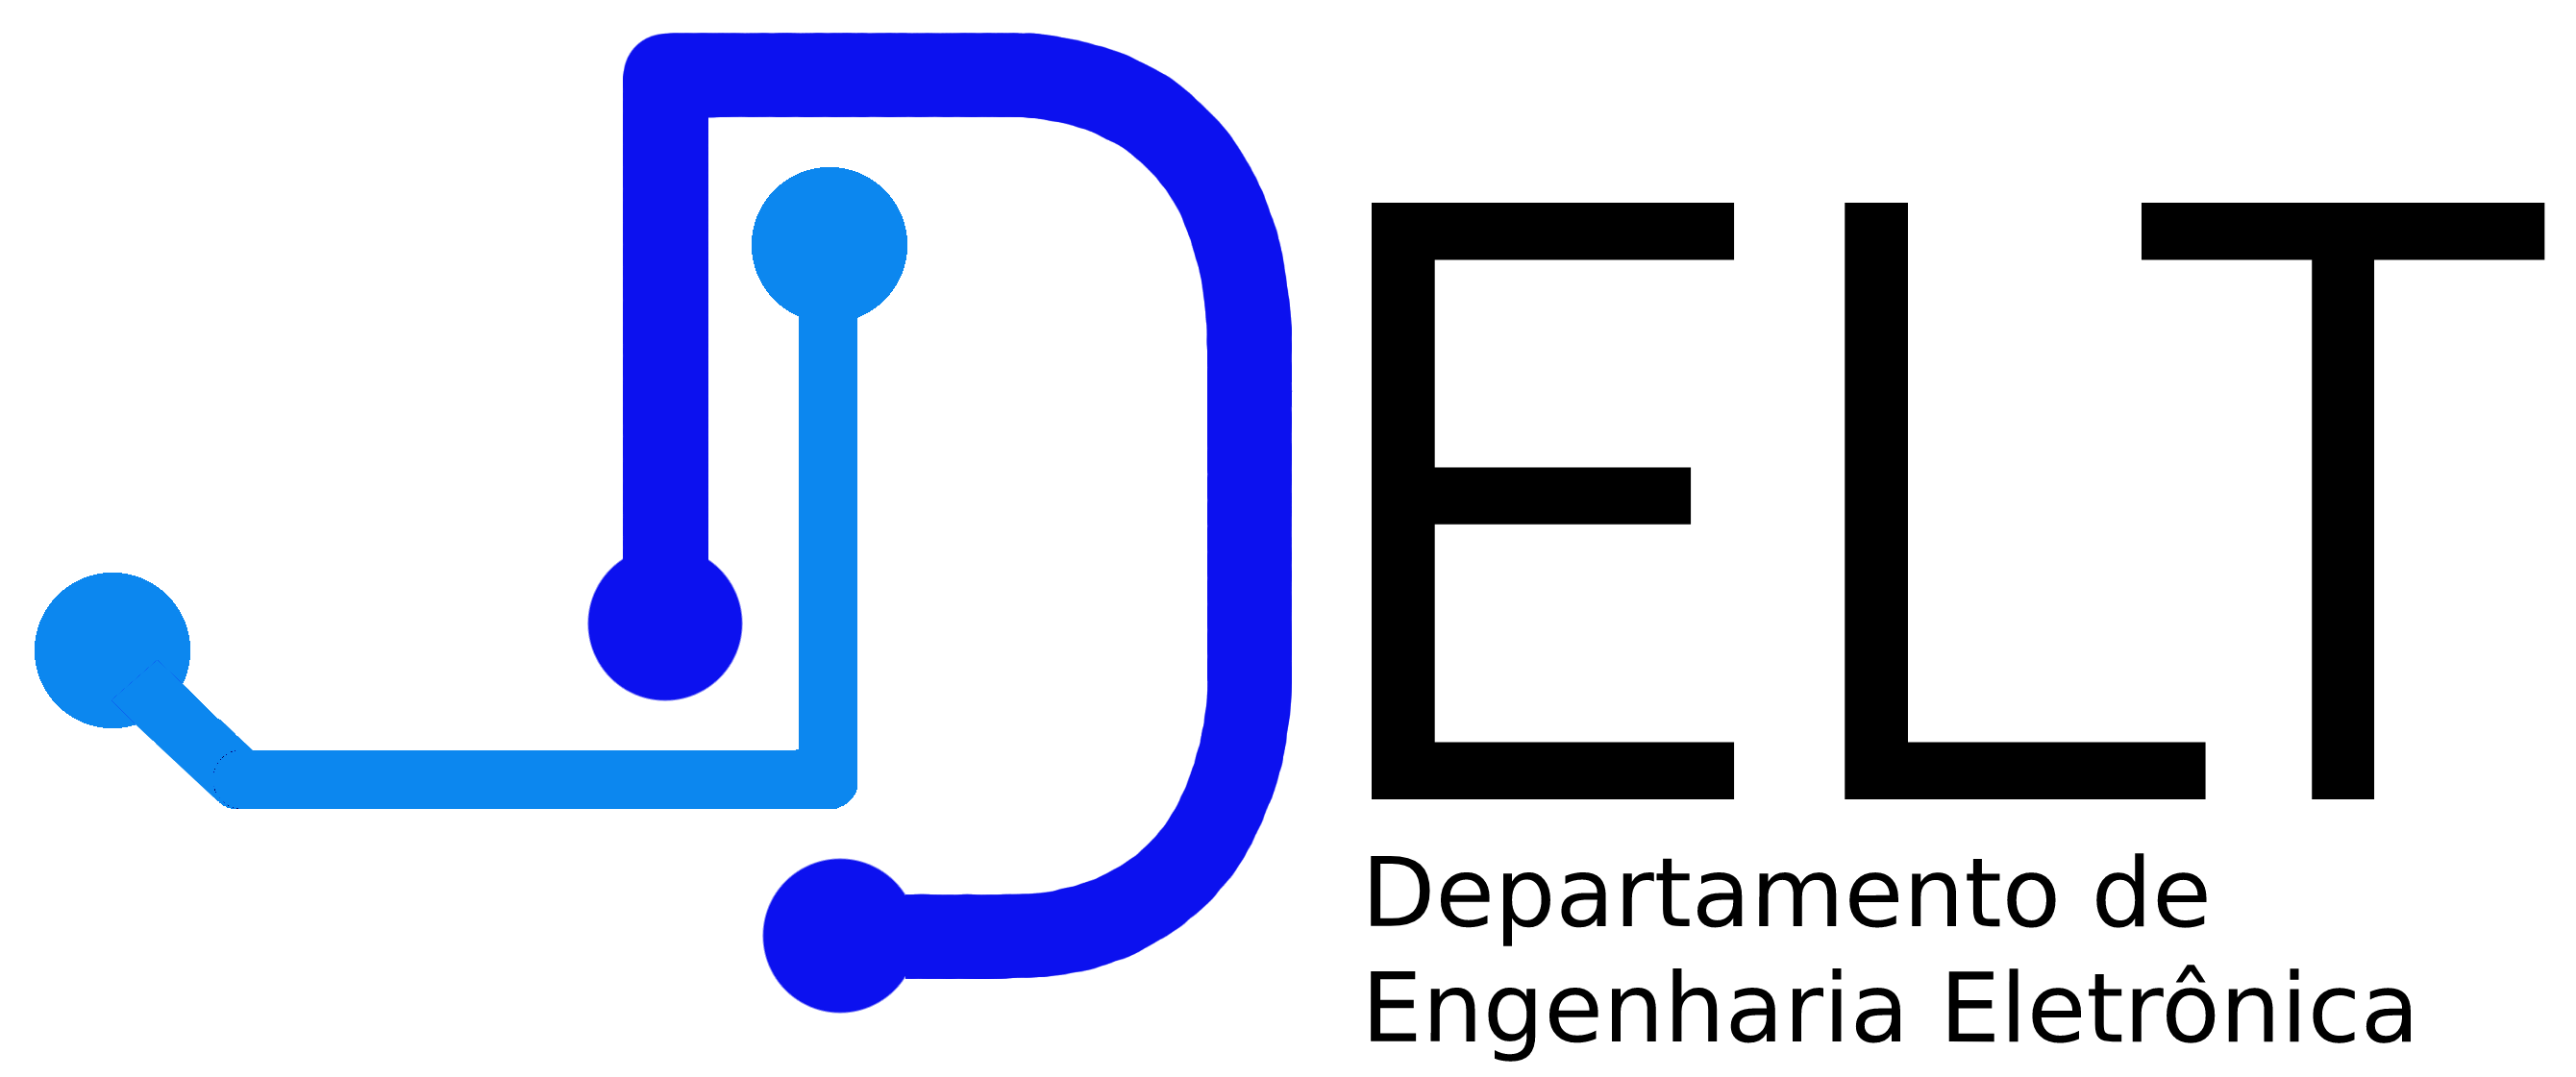
\includegraphics[width=3.8cm]{figures/delt_logo.png}
    
    % ====== Instituição ======
    \vspace{2.8cm}
    {\Large \textbf{\universidade}}\\[0.4cm]
    {\large \departamento}\\[0.3cm]
    {\large \curso}\\[3.5cm]
    
    % ====== Título ======
    {\LARGE \textbf{\titulo}}\\[4cm]
    
    % ====== Nome, disciplina e professor ======
    {\large \textbf{\autor}}\\[0.3cm]
    {\large \textit{\disciplina}}\\[0.3cm]
    {\large \professor}\\[4cm]
    
    % ====== Rodapé da capa ======
    {\large \local}\\[0.2cm]
    {\large \dataentrega}
    
    \end{center}
\end{titlepage}

% ============================
% Sumário
% ============================
\tableofcontents
\newpage

% ============================
% Corpo do relatório
% ============================

\section{Introdução}

O problema de planejamento de movimento consiste em encontrar uma trajetória
livre de colisões entre uma configuração inicial e uma configuração final. Para
um corpo rígido livre no espaço, a configuração envolve simultaneamente posição
e orientação. Por isso, neste trabalho a configuração do robô é representada em
\(SE(3)\), o grupo das transformações rígidas no espaço
\cite{LynchPark2017}.

Métodos baseados em amostragem, como o RRT, são adequados para problemas de
planejamento em espaços de configuração de maior dimensão, pois evitam a
construção explícita de todo o espaço livre \cite{LaValle2006,Choset2005}.
Neste trabalho, foi implementado um planejador RRT bidirecional em \(SE(3)\)
para um corpo rígido. O caminho planejado é posteriormente usado como referência
para seguimento por campo vetorial.

\section{Planejamento de movimento em \texorpdfstring{$SE(3)$}{SE(3)}}

\subsection{Representação da configuração}

O robô é tratado como um corpo rígido livre. Sua pose é representada por uma
matriz homogênea
\[
H =
\begin{bmatrix}
R & p \\
0 & 1
\end{bmatrix}
\in SE(3),
\]
em que \(R \in SO(3)\) representa a orientação e
\(p \in \mathbb{R}^3\) representa a posição. Essa representação permite tratar
posição e orientação como uma única configuração do corpo rígido
\cite{LynchPark2017,Murray1994,Barfoot2017}.

\subsection{Métrica utilizada}

Para comparar duas poses \(H_1\) e \(H_2\), a implementação utiliza o erro
relativo
\[
H_{\mathrm{rel}} = H_1^{-1}H_2.
\]
Esse erro relativo é levado para a álgebra de Lie por meio do logaritmo
matricial:
\[
\hat{\xi}
=
\log(H_1^{-1}H_2),
\qquad
\xi
=
\vee\left(\log(H_1^{-1}H_2)\right).
\]
No código, a convenção adotada para o vetor de twist é
\[
\xi =
\begin{bmatrix}
v \\
\omega
\end{bmatrix},
\]
isto é, a parte linear \(v\) vem antes da parte angular \(\omega\).

Como o vetor \(\xi\) combina componentes translacionais e rotacionais, foi usada
a matriz de ponderação
\[
G_\ell =
\mathrm{diag}(1,1,1,\ell^2,\ell^2,\ell^2).
\]
O parâmetro \(\ell\) é uma escala de comprimento usada para ponderar a parte
angular em relação à parte translacional. A métrica utilizada no planejador é
\[
d(H_1,H_2)
=
\sqrt{
\xi^\top G_\ell \xi
}.
\]
Essa métrica foi usada para a busca do nó mais próximo, para o avanço do
planejador, para a checagem e discretização de arestas e para a discretização do
caminho final. A necessidade de ponderar translação e rotação em movimentos
rígidos é discutida por Park \cite{Park1995}; a formulação por twists,
exponencial e logaritmo segue a representação usual de \(SE(3)\)
\cite{LynchPark2017,Barfoot2017}.

\subsection{Interpolação e avanço}

A interpolação entre duas poses é calculada diretamente em \(SE(3)\) por
\[
H(s)
=
H_1
\exp\left(
s\log(H_1^{-1}H_2)
\right),
\qquad
s\in[0,1].
\]
Essa interpolação utiliza o movimento relativo entre as poses e evita a
parametrização da orientação por ângulos de Euler
\cite{LynchPark2017,Barfoot2017}.

O operador de avanço usado pelo RRT segue a mesma construção. Dado um nó próximo
\(H_{\mathrm{near}}\) e uma pose alvo \(H_{\mathrm{target}}\), a nova pose é
definida por
\[
H_{\mathrm{new}}
=
H_{\mathrm{near}}
\exp\left(
\alpha
\log(H_{\mathrm{near}}^{-1}H_{\mathrm{target}})
\right),
\]
com
\[
\alpha =
\min\left(
1,
\frac{\eta}{d(H_{\mathrm{near}},H_{\mathrm{target}})}
\right).
\]
Se o alvo está dentro do passo máximo, o novo nó coincide com o alvo. Caso
contrário, o novo nó avança apenas até a distância máxima \(\eta\), medida pela
métrica definida anteriormente.

\subsection{RRT bidirecional}

O planejador implementado é um RRT bidirecional com estratégia do tipo
RRT-Connect. São mantidas duas árvores: \(T_{\mathrm{start}}\), inicializada em
\(H_{\mathrm{start}}\), e \(T_{\mathrm{goal}}\), inicializada em
\(H_{\mathrm{goal}}\). A cada iteração, uma árvore é expandida e a outra é usada
como referência para tentativa de conexão.

\begin{algorithm}[H]
\caption{RRT bidirecional em \(SE(3)\)}
\label{alg:rrt_se3_bidirectional}
\begin{algorithmic}[1]
\Require \(H_{\mathrm{start}}\), \(H_{\mathrm{goal}}\), limites de amostragem, métrica \(d(\cdot,\cdot)\), passo \(\eta\)
\Ensure Caminho discretizado livre de colisões ou falha
\State Inicializar \(T_{\mathrm{start}}\) com \(H_{\mathrm{start}}\)
\State Inicializar \(T_{\mathrm{goal}}\) com \(H_{\mathrm{goal}}\)
\For{\(k = 1,\ldots,N_{\max}\)}
    \State Selecionar a árvore ativa \(T_a\) e a árvore oposta \(T_b\)
    \State Amostrar uma configuração \(H_{\mathrm{rand}}\) em \(SE(3)\)
    \State Encontrar \(H_{\mathrm{near}}\in T_a\) mais próximo de \(H_{\mathrm{rand}}\)
    \State Calcular \(H_{\mathrm{new}}\) pelo avanço em \(SE(3)\)
    \If{\(H_{\mathrm{new}}\) é livre e a aresta \((H_{\mathrm{near}},H_{\mathrm{new}})\) é livre}
        \State Adicionar \(H_{\mathrm{new}}\) em \(T_a\)
        \State Tentar conectar \(T_b\) a \(H_{\mathrm{new}}\)
        \If{as árvores foram conectadas}
            \State Reconstruir o caminho entre \(H_{\mathrm{start}}\) e \(H_{\mathrm{goal}}\)
            \State Aplicar pós-processamento por shortcut
            \State Discretizar o caminho final
            \State \Return caminho discretizado
        \EndIf
    \EndIf
    \State Alternar os papéis de \(T_a\) e \(T_b\)
\EndFor
\State \Return falha
\end{algorithmic}
\end{algorithm}

Na implementação, a amostragem possui termos de viés para favorecer a conexão
entre as árvores. Com uma certa probabilidade, o alvo da expansão é escolhido
como um nó da árvore oposta; com outra probabilidade, é escolhida a raiz da
árvore oposta. Caso contrário, uma nova configuração é amostrada no espaço de
busca. A posição é amostrada em uma caixa limitada e a orientação é amostrada em
\(SO(3)\). Essa estrutura segue os princípios de RRT e RRT-Connect para
planejamento de movimento \cite{LaValle2006,Choset2005,KuffnerLaValle2000}.

\subsection{Oráculo de colisão}

O robô é representado por primitivas geométricas no frame local do corpo. Para
uma pose \(H\), cada primitiva local é transformada para o mundo por
\[
H_{\mathrm{obj}} = H H_{\mathrm{local}}.
\]
Depois da transformação, calcula-se a AABB de cada primitiva. Essas caixas são
usadas como etapa de broad phase, de modo que apenas pares candidatos sejam
avaliados pela rotina de distância geométrica. A pose é considerada em colisão
quando a distância entre primitivas é menor que uma tolerância
\(d_{\mathrm{tol}}\).

\subsection{Discretização de arestas}

Verificar apenas os nós da árvore não basta, pois o movimento entre duas poses
livres pode cruzar obstáculos. Assim, cada aresta é discretizada de acordo com a
métrica em \(SE(3)\):
\[
n =
\left\lceil
\frac{d(H_1,H_2)}{\Delta_{\mathrm{edge}}}
\right\rceil.
\]
As poses intermediárias são geradas por
\[
H_i =
H_1
\exp\left(
s_i\log(H_1^{-1}H_2)
\right),
\qquad
s_i = \frac{i}{n}.
\]
O parâmetro \(\Delta_{\mathrm{edge}}\) é usado para a checagem de colisão ao
longo das arestas. Já \(\Delta_{\mathrm{out}}\) é usado apenas para discretizar
o caminho final retornado.

\subsection{Pós-processamento por shortcut}

O caminho bruto produzido pelo RRT pode conter desvios desnecessários. Por isso,
foi implementado um pós-processamento por shortcut. O procedimento escolhe dois
waypoints do caminho e testa a conexão direta entre eles. Se essa conexão direta
estiver livre de colisão, os waypoints intermediários são removidos. Esse
procedimento tende a reduzir o caminho, mas não garante otimalidade global
\cite{LaValle2006,Choset2005}.

\subsection{Seguimento por campo vetorial}

Depois do planejamento, o caminho discretizado é usado como curva de referência
para um campo vetorial em \(SE(3)\). O campo vetorial fornece diretamente um
twist desejado
\[
\xi_d =
\begin{bmatrix}
v_d \\
\omega_d
\end{bmatrix},
\]
que é aplicado ao modelo cinemático do corpo rígido. Essa abordagem é compatível
com formulações de seguimento de caminhos em grupos de Lie, como discutido por
Bartelt et al. \cite{Bartelt2026}, especialmente em \(SE(3)\), onde a entrada
pode ser interpretada como o twist mecânico do corpo.

De forma geral, o campo vetorial combina uma componente de convergência para a
curva com uma componente de avanço ao longo da curva. No código, o twist
retornado pelo campo vetorial é modulado por um fator escalar \(\alpha\),
definido em função da distância até a pose final:
\[
\alpha(d)
=
1
-
e^{-\lambda d}
\left(
1+\lambda d
\right),
\]
em que
\[
d =
\left\|
\log\left(
H^{-1}H_{\mathrm{goal}}
\right)
\right\|.
\]
Quando o corpo está longe do alvo, \(\alpha(d)\) fica próximo de \(1\), de modo
que o campo vetorial praticamente não é alterado. Quando o corpo se aproxima da
pose final, \(\alpha(d)\) tende a \(0\), reduzindo gradualmente o twist desejado.
Isso suaviza a chegada e evita que o robô continue avançando com velocidade
significativa perto da pose final. O twist aplicado é
\[
\xi =
\alpha(d)\xi_d.
\]

\subsection{Resumo da implementação}

O núcleo do planejador foi implementado em C++ e é chamado por uma interface
Python. O resultado retorna sucesso ou falha, caminho por waypoints, caminho
discretizado, número de iterações, número de nós nas árvores e tempos de
execução. O caminho discretizado é usado pelo campo vetorial para gerar o
movimento do corpo rígido.

\section{Resultados preliminares}

O cenário considerado contém um corpo rígido representando um UAV. Os obstáculos
são compostos por caixas e cilindros. O RRT bidirecional foi usado para conectar
uma pose inicial a uma pose alvo em \(SE(3)\). O caminho retornado pelo
planejador foi pós-processado por shortcut e, em seguida, discretizado para ser
usado como referência pelo campo vetorial. A simulação em UAIBot mostra o
caminho planejado e o caminho seguido pelo corpo rígido.

Para avaliar o tempo de execução do planejador, foi realizado um benchmark com
100 execuções independentes do mesmo problema de planejamento. Não foi fixada
semente aleatória, de modo que as variações observadas refletem a natureza
amostral do RRT. Em todas as execuções, foram mantidos os mesmos parâmetros de
planejamento, o mesmo modelo geométrico do corpo rígido e o mesmo conjunto de
obstáculos.

Das 100 execuções realizadas, o planejador obteve sucesso em 100 casos e não
apresentou falhas. Assim, a taxa de sucesso observada no cenário testado foi de
\[
\frac{100}{100} = 100{,}00\%.
\]
Considerando apenas as execuções bem-sucedidas, o tempo médio de execução foi
\[
\bar{t}_{\mathrm{exec}} = 0{,}022736\,\mathrm{s},
\]
com desvio padrão
\[
\sigma_{t} = 0{,}010538\,\mathrm{s}.
\]
Em milissegundos, esses valores correspondem aproximadamente a
\(22{,}736\,\mathrm{ms}\) de média e \(10{,}538\,\mathrm{ms}\) de desvio padrão.

Os resultados indicam que, para o cenário considerado, o planejador foi capaz de
encontrar caminhos livres de colisão de forma consistente. A variação no tempo
de execução é esperada, pois o RRT bidirecional é baseado em amostragem
aleatória. Assim, diferentes execuções podem gerar árvores distintas e encontrar
conexões em momentos diferentes da busca.

Essa avaliação é preliminar e tem como objetivo caracterizar o comportamento do
planejador no cenário implementado. Uma análise mais ampla poderia considerar
outros ambientes, diferentes resoluções de checagem de arestas e diferentes
parâmetros de amostragem.

\section{Conclusão preliminar}

Foi implementado um pipeline de planejamento para corpo rígido em \(SE(3)\). A
métrica logarítmica ponderada permitiu combinar posição e orientação na busca, e
o RRT bidirecional encontrou um caminho livre de colisões no cenário avaliado. A
discretização de arestas foi usada para verificar o movimento entre poses, e o
pós-processamento por shortcut reduziu desvios do caminho bruto.

O caminho discretizado foi usado como referência para seguimento por campo
vetorial. A modulação do twist desejado reduziu a velocidade próxima ao alvo,
suavizando a chegada à pose final. O método implementado, portanto, integra
planejamento em \(SE(3)\), verificação de colisão e seguimento de caminho para um
corpo rígido livre.

\bibliographystyle{plain}
\bibliography{references}

\end{document}
